\documentclass[conference]{IEEEtran}
\IEEEoverridecommandlockouts
\usepackage{cite}
\usepackage{amsmath,amssymb,amsfonts}
\usepackage{algorithmic}
\usepackage{graphicx}
\usepackage{textcomp}
\usepackage{xcolor}
\usepackage{multirow}
\def\BibTeX{{\rm B\kern-.05em{\sc i\kern-.025em b}\kern-.08em
    T\kern-.1667em\lower.7ex\hbox{E}\kern-.125emX}}
\begin{document}

\title{Smart Spreading Factor Assignment for LoRaWANs}


\author{\IEEEauthorblockN{Tugrul Yatagan\IEEEauthorrefmark{1} and Sema F. Oktug\IEEEauthorrefmark{2}}
\IEEEauthorblockA{Department of Computer Engineering,
Istanbul Technical University\\
Istanbul, Turkey\\
Email: \IEEEauthorrefmark{1}yatagan@itu.edu.tr, \IEEEauthorrefmark{2}oktug@itu.edu.tr}}
\maketitle


\begin{abstract}
Low power wide area network (LPWAN) technologies offer affordable connectivity to massive number of low-power devices distributed over very large geographical areas using license-free frequency bands. Focus on this work is one of the most promising LPWAN technologies: LoRa. LoRa offers long range communication and strong resilience to interference by proprietary modulation technique based on Chirp Spread Spectrum. LoRa trades data rate for sensitivity and communication range by spreading symbols within a fixed channel bandwidth. Spreading factor (SF) assignment of nodes has strong effect on collisions thus network performance. In this work, we implemented a simulation environment to study different SF assignment schemes and we proposed a machine learning technique to optimize SF assignment. Finally, we illustrate simulation results for proposed machine learning SF assignment technique.
\end{abstract}


\begin{IEEEkeywords}
LoRa, Spreading Factor, IoT, LPWAN, Machine Learning
\end{IEEEkeywords}


\section{Introduction}
\par In the last few years, number of Internet of Things applications increase exponentially. \cite{7721743} Recent developments on LPWAN technologies has great impact on IoT application number growth. LPWAN technologies offer solutions to some of the oldest wireless communication challenges. Traditional wireless communication methods such as cellular networks (e.g., 2G, 3G, LTE) and short-range communication methods (e.g., Bluetooth, WiFi, Zigbee) cannot provide low power and long range at the same time. [CITE] Cellular networks can provide long range and high data rate but they are complex and consume too much power. Besides, most of the IoT applications don't require high data rate. Short-range communication methods can provide relatively low power consumption but their range is limited to a few hundred meters at best. \cite{7815384} LPWAN technologies fill the technology gap between short range and cellular communication by providing low power and long range communication. LPWAN technologies basically sacrifice data rate to provide low power consumption.

\par There are several emerging LPWAN technologies. LoRa, Sigfox, NB-IoT and LTE-M are commonly used, well known LPWAN technologies. LoRa and Sigfox use license free ISM frequency bands while NB-IoT and LTE-M use licensed frequency bands which brings extra cost. [CITE] Both LoRa and Sigfox known for ultra low power consumption and resilient to interference while NB-IoT and LTE-M are promoted for higher data rate. LoRa has open standard MAC protocol called LoRaWAN. [CITE] LoRaWAN and Sigfox MAC protocols are based on pure ALOHA medium access. [CITE] LoRaWAN networks can be deployed as private network. However, Sigfox and NB-IoT supports only operator contracted deployments. [CITE] Number of messages that Sigfox end device can send in a day is limited to 140 packets for uplink and just 4 packets for downlink. Sigfox packet payload is limited to 12 bytes for uplink and 8 bytes for downlink. [CITE] However LoRa supports up to 243 bytes payload and NB-IoT supports up to 1600 bytes payload. [CITE] Sigfox maximum data rate is also very low 100 bps, on the other hand maximum data rate for LoRa and NB-IoT are 50 kbps and 200 kbps respectively. [CITE]

\par LoRa can adjust data rate by spreading symbols within a fixed channel bandwidth. This enables tradeoff between receive sensitivity and transmission air time. [CITE] LoRa supports 6 different SF option. Simultaneous same SF transmissions are prone to collision however different SF transmissions in same channel are orthogonal to each other, thus SF assignment is crucial for overall network performance. [CITE] In this work, we introduce a custom made LoRa discrete event simulator to study LoRa SF assignment issue. We also proposed an SF assignment scheme to increase network performance with the help of machine learning methods and we verified our proposal using our simulator.

\par The following two sections provides an background information about LoRaWAN and LoRa. Section \ref{Other Related Works} describes other related works. Section \ref{Proposed Technique} describes proposed technique for SF assignment. Simulation environments and results are shown in Section \ref{Simulation Environment and Results}. Finally, Section \ref{Conclusion} concludes the paper.


\section{LoRaWAN} \label{LoRaWAN}
\par LoRa is a wireless link technology for LPWAN applications. LoRa has an open standard MAC protocol called LoRaWAN. LoRa and LoRaWAN terms are frequently and incorrectly used for each other.

\par LoRaWAN is a medium access control (MAC) layer protocol which designed for large scale LoRa networks. LoRaWAN is an open source standard developed and maintained by LoRa Alliance. LoRa Alliance is an open, non-profit organization dedicated to standardization of LoRaWAN. LoRa can be used without LoRaWAN as a wireless link technology, however LoRaWAN is developed considering well known LPWAN challenges and their best practice solutions. LoRaWAN also provides inter-operability between different LoRa networks. LoRaWAN is based on pure ALOHA medium access. LoRaWAN provides lightweight but powerful standard for wide range of LoRa IoT applications.

\par A typical LoRaWAN network consist of three network entities.

\subsection{End node}
\par LoRaWAN end node (EN) is low power embedded device that communicates to gateways. LoRaWAN standard defines three classes for end devices which are Class A, Class B, and Class C for providing LPWAN solution to different scenarios. Class A end nodes generates uplink transmission at any time and only receives a period of time after uplink transmission. Class B end nodes extend Class A by adding scheduled receive windows for downlink transmission. Receive window is synchronized using beacon packet transmitted by gateway. Class C end nodes extend Class A by keeping receive window open unless they are transmitting. This provides low latency donwlink communication but requires more power consumption. [CITE] In this paper, we focused on Class A end devices since Class A provides lowest power consumption.

\subsection{Gateway}
\par LoRaWAN gateway (GW) is device that receive/transmit packets coming from/to end nodes. A typical gateway can receive from multiple channel at the same time. Gateways are typically connected to power grid so power consumption of a gateway is insignificant most of the deployments.

\subsection{Network server}
\par LoRaWAN network server (NS) is server that provides MAC layer processing. Network server routes messages from application to end nodes, and vice versa. Network server can be used for tweaking end node parameters like channel, transmit power, SF to increase network performance.


\section{LoRa}
\par LoRa is the name of the proprietary physical layer radio and chipset technology that provides wireless link solution for low power wide area networks. LoRa is designed and patented by Semtech Corporation. LoRa uses proprietary spread spectrum modulation technique that is derivative of Chirp Spread Spectrum (CSS). Chirp is a sinusoidal signal which its  frequency increases over time. The chirp frequency increases linearly and sweeps entire bandwidth. [CITE] We invite readers to refer to \cite{AN1200.22} for further details.

\subsection{Spreading Factor}
\par Spreading factor (SF) is the ratio between symbol rate and chip rate. The ratio between symbol and chip rate is equal to $2$\textsuperscript{SF}. SF can take values between 7 to 12. SF also determines data rate of a LoRa transmission \cite{AN1200.22}.

\begin{equation} \label{eq:bit_rate_sf}
R_{b} = SF * \dfrac{\left[ \dfrac{4}{4+CR} \right] }{ \left[ \dfrac{2^{SF}}{BW} \right]} \ bits/sec
\end{equation}

Where, SF is spreading factor $SF \in \{7,..,12\}$, CR is error correction code rate $CR \in \{1,..,4\}$ and $BW$ is bandwidth in Hertz \cite{AN1200.22}.

\par While BW and CR are constant, as the SF increases the data rate decreases. Increasing SF makes the signal more resilient to noise thus increases the transmission range. Increasing SF also increases transmission duration which increases power consumption. Therefore it is possible to trade between data rate, range and power consumption by  changing SF.

\subsection{Spreading Factor Assignment Issue}
\par Simultaneous different SF transmissions are orthogonal to each other up to some extent. Which means, a LoRa gateway can simultaneously receive multiple transmissions with different SFs. However, simultaneous transmissions with same SF may not be received by gateway due to collision. For this reason, spreading factor assignment of nodes is crucial for network performance.

\par Initially, a node is not aware of how far it is from a GW. However, a node can guess how far away from the gateway by observing received signal power of a downlink transmission. If a downlink transmission received signal power is too high then node can decrease its next transmission SF or transmit power to decrease power consumption. Also GW can request from a node to decrease node's SF or transmit power. This SF assignment method is called lowest possible SF assignment scheme for the rest of the paper.

\par In Figure~\ref{fig:collision}, a LoRaWAN network distributed around a single GW is illustrated. Different color rings represent achievable range of different SF from GW and different color circles represent nodes with selected SF. Most of the end devices which close to the GW will fall into lowest SF (SF7) area section. End devices which close to the GW will probably select lowest SF all the time. Which results a lot of collisions between same SF transmissions. Collision number increases while end device number close to the GW increases.

\begin{figure}
\centering
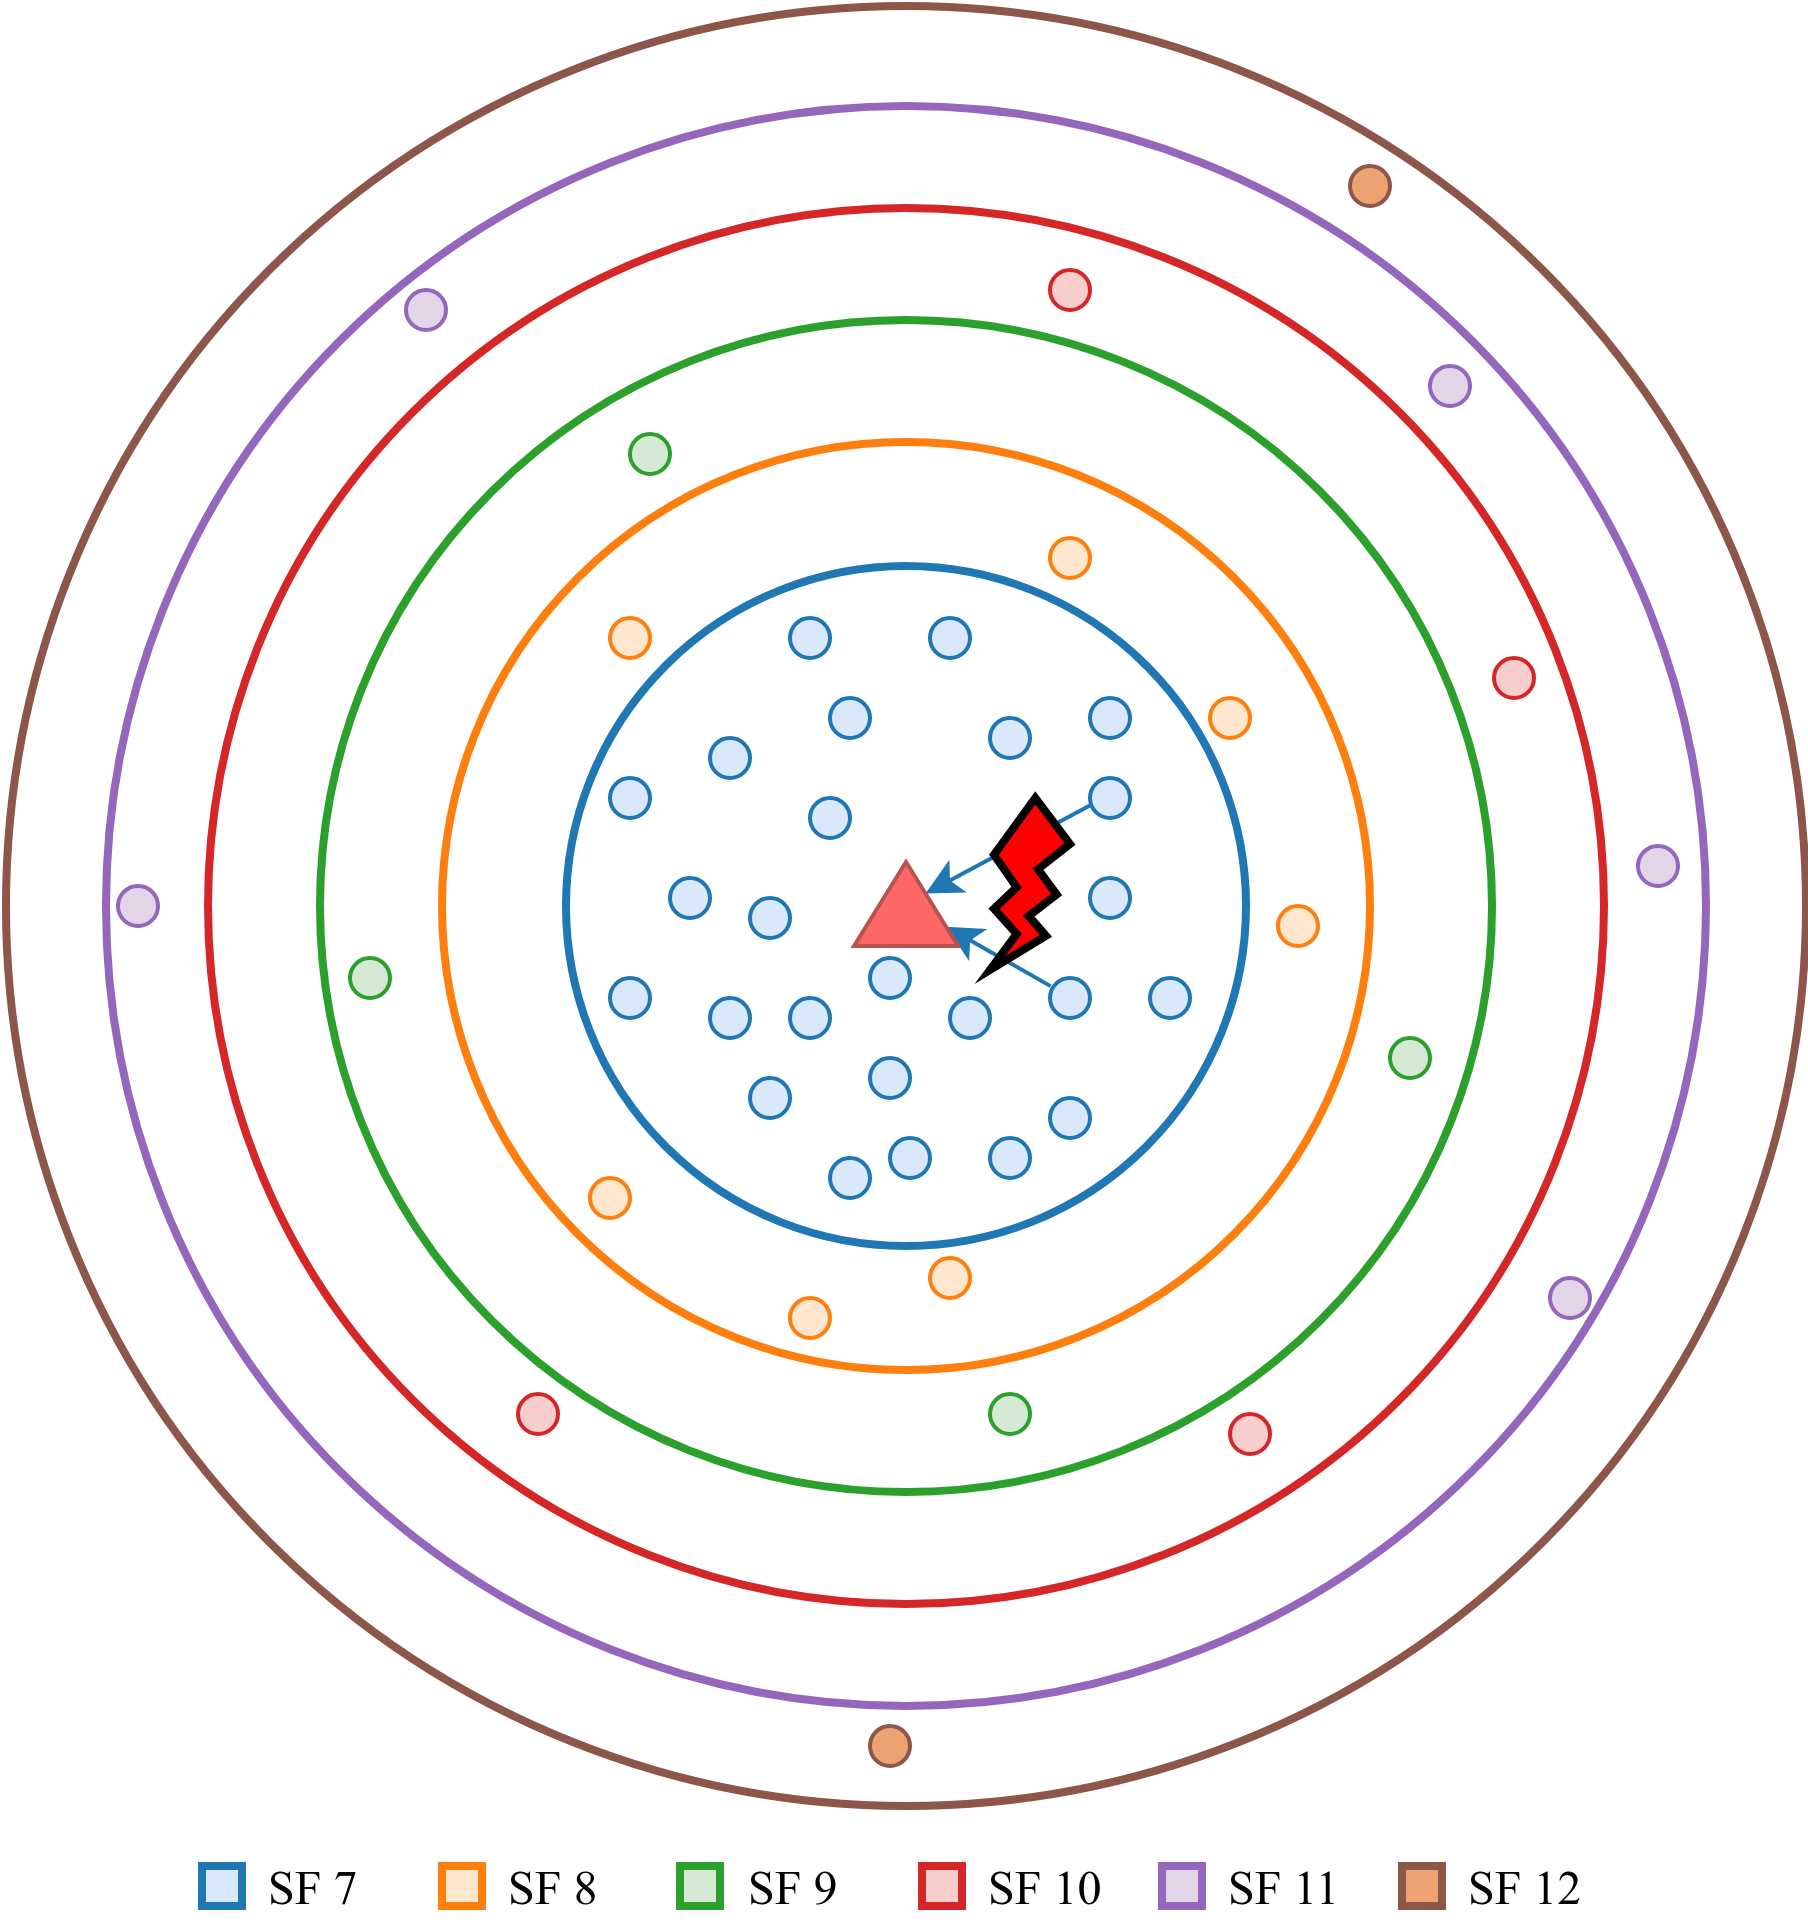
\includegraphics[width=0.5\textwidth]{collision}
\caption{Collision between nodes close to the GW.}
\label{fig:collision}
\end{figure}


\section{Other Related Works} \label{Other Related Works}
The literature related to the work presented in this paper has started growing recently. LPWAN technologies and especially LoRa/LoRaWAN attract researchers attention lately. We listed some of these works which studying LoRaWAN and LoRa SF.

\par In \cite{7996384}, the authors evaluated the performance of LoRa networks in a smart city scenario. The
authors proposed a link measurement and a link performance model for LoRa. The authors also proposed a SINR threshold matrix for modeling LoRa interference between simultaneous but different SF LoRa transmissions. They implement a LoRa simulator in ns-3 to study scalability and performance of LoRaWAN networks. Their results show that LoRaWAN networks scale well as the number of nodes and gateways increases. They also show that SF assignment has great effect on network performance.

\par In \cite{8090518}, another LoRaWAN ns-3 simulator is presented. Authors introduced an error model for determining range as well as interference between multiple simultaneous LoRa transmissions. Their simulator supports LoRaWAN Class A end devices, multiple gateways, both upstream and downstream confirmed messages. Their results show that allocating network parameters to end devices is hugely important for the performance of LoRaWAN networks.

\par In \cite{s17061193}, the authors investigated single gateway LoRaWAN network scalability in terms of the number of end nodes using a simulation model based on real measurements. They measure the impact of two concurrent LoRa transmissions on each other by using physical LoRaWAN end devices and a gateway then they created a simulation model from measurements. Their results show that LoRaWAN has better scalability than pure ALOHA since a LoRa packet may still go through under collision if the the last six symbols of preamble and header of the packet does not collide.

\par In \cite{8267219}, the authors studied imperfect orthogonality between different LoRa SF transmissions. The authors state that a LoRa transmission can be interfered even between different SF transmissions when power of the interfering signal significantly overcomes the reference signal. Their experimental results show that this power difference is around 16 dB and this power difference can be seen when  interferer is close to receiver or multiple interferer can create this power difference cumulatively. 

\par In \cite{8430542}, the authors investigated the impact of interference caused by simultaneous LoRa transmissions using the same SF as well as different SFs. They derived aggregated co-SF and inter-SF interference power SIR distributions to capture the coverage performance with respect to the distance from the gateway for modeling interference in multiple gateway scenarios. Their results show that transmission among different SFs can cause a significant impact in high-density LoRaWAN networks.


\section{Proposed Technique} \label{Proposed Technique}
\par The collision issue illustrated in Figure~\ref{fig:collision} can be solved if the GW force some of the close end nodes to select higher SF even if they can able to communicate with lower SF. This may result lower collisions due to the orthogonality of different SF as shown in Figure~\ref{fig:collision_solution_single_gw}. Higher SF assigned nodes are drawn with bold circle border in Figure~\ref{fig:collision_solution_single_gw}. However, how GW assign SF to which node becomes an another issue. Increasing a node's SF should be done carefully since higher SF means higher time on air and higher time on air is more prone to collision with other higher SF transmissions. In multiple GW scenarios, this approach may increase the collision number with nodes in other GW's range. Thus, extra care must be taken for nodes in intersection area of GWs illustrated in Figure~\ref{fig:collision_solution_multi_gw}.

\par It is difficult to propose a single SF assignment rule for every possible LoRaWAN topology since every network is different and optimizing their nodes SFs requires different rules. For this reason, we proposed a machine learning based SF assignment scheme to decrease same SF transmission collision number.  This technique learns nodes behavior of a network. A NS can keep track of successful uplink transmission from nodes and their SFs. NS can also keep track of some of the collided transmission if header part of the packet does not interfered at GW. However, NS cannot keep track of transmissions with receive power lower than GW sensitivity. Using these obtained information NS can train a classifier for predicting transmission result for specific node and specific SF input. Using this predictor GWs can assign the lowest possible SF to nodes considering the collision probability.

\par In this work, we used decision tree classifier to predict transmission results. We utilized Gini index criteria to measure quality of decision tree splits and used balanced class weights. As most of the machine learning applications, increasing data set size increases prediction accuracy. For our case, data set size is directly proportional to simulation duration. Thus increasing simulation duration, increases the prediction accuracy. For real world cases, NS can keep track of transmission and it can create a classifier daily basis, then GW can request from nodes to use this new SF.

\begin{figure}
\centering
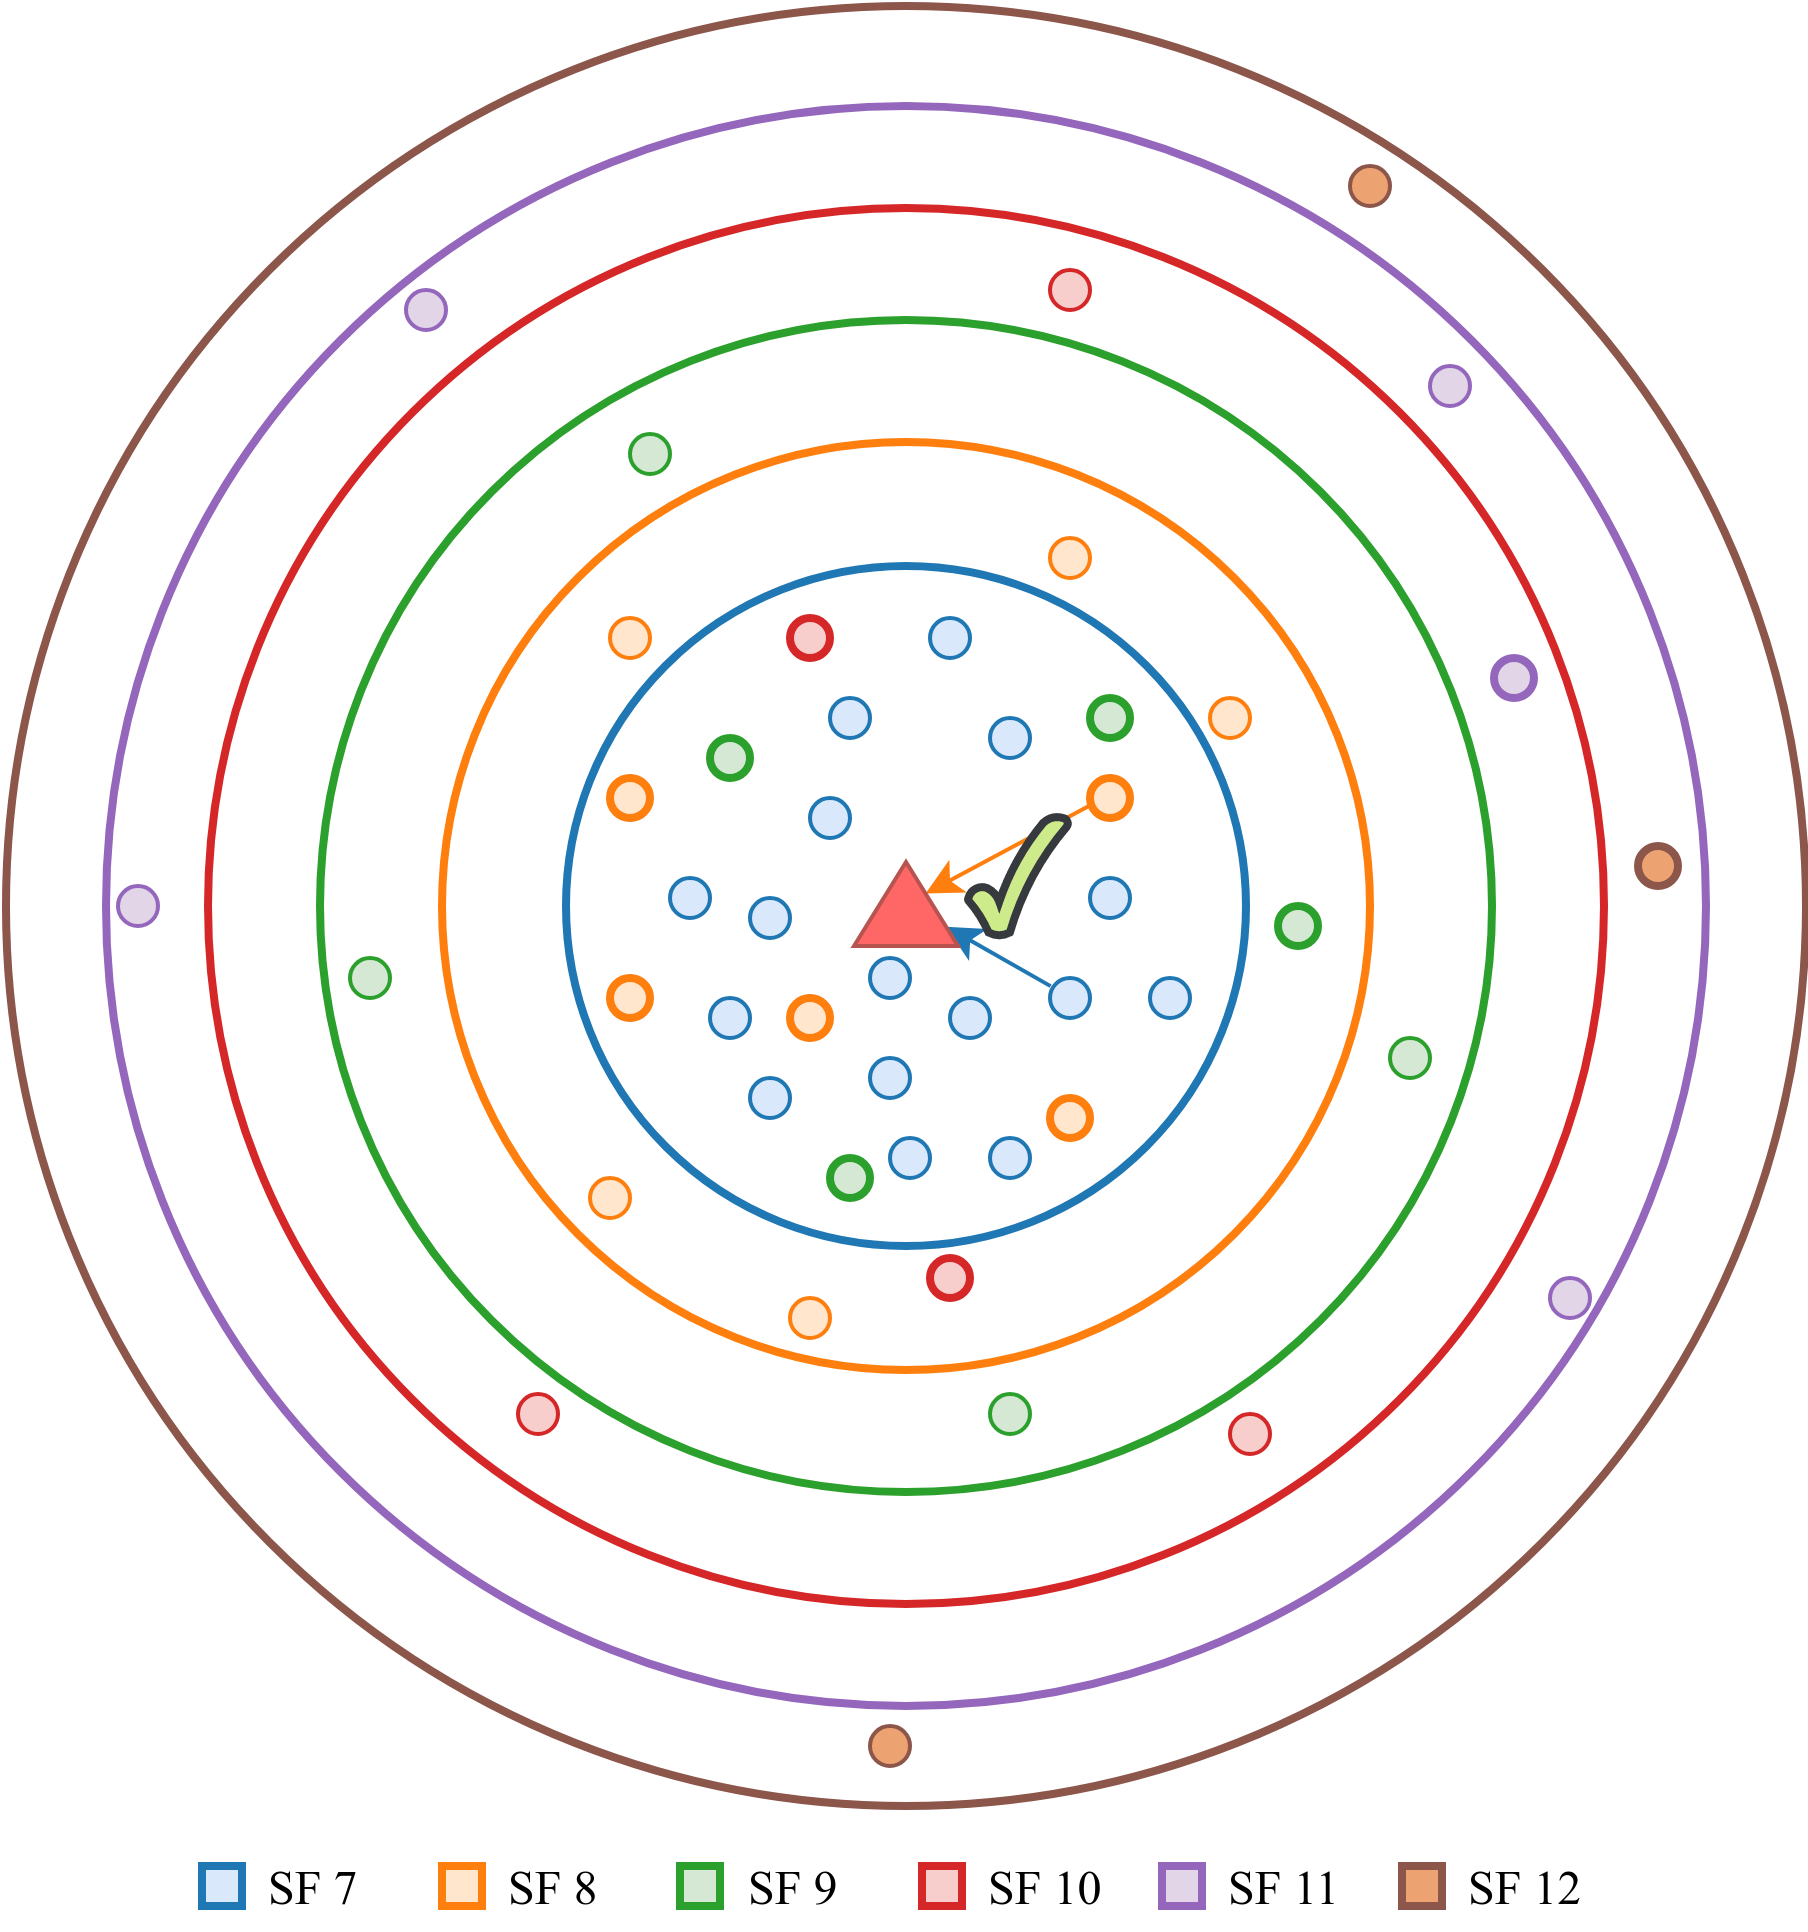
\includegraphics[width=0.5\textwidth]{collision_solution_single_gw}
\caption{Collision between nodes close to the GW can be prevented by using higher SF.}
\label{fig:collision_solution_single_gw}
\end{figure}

\begin{figure}
\centering
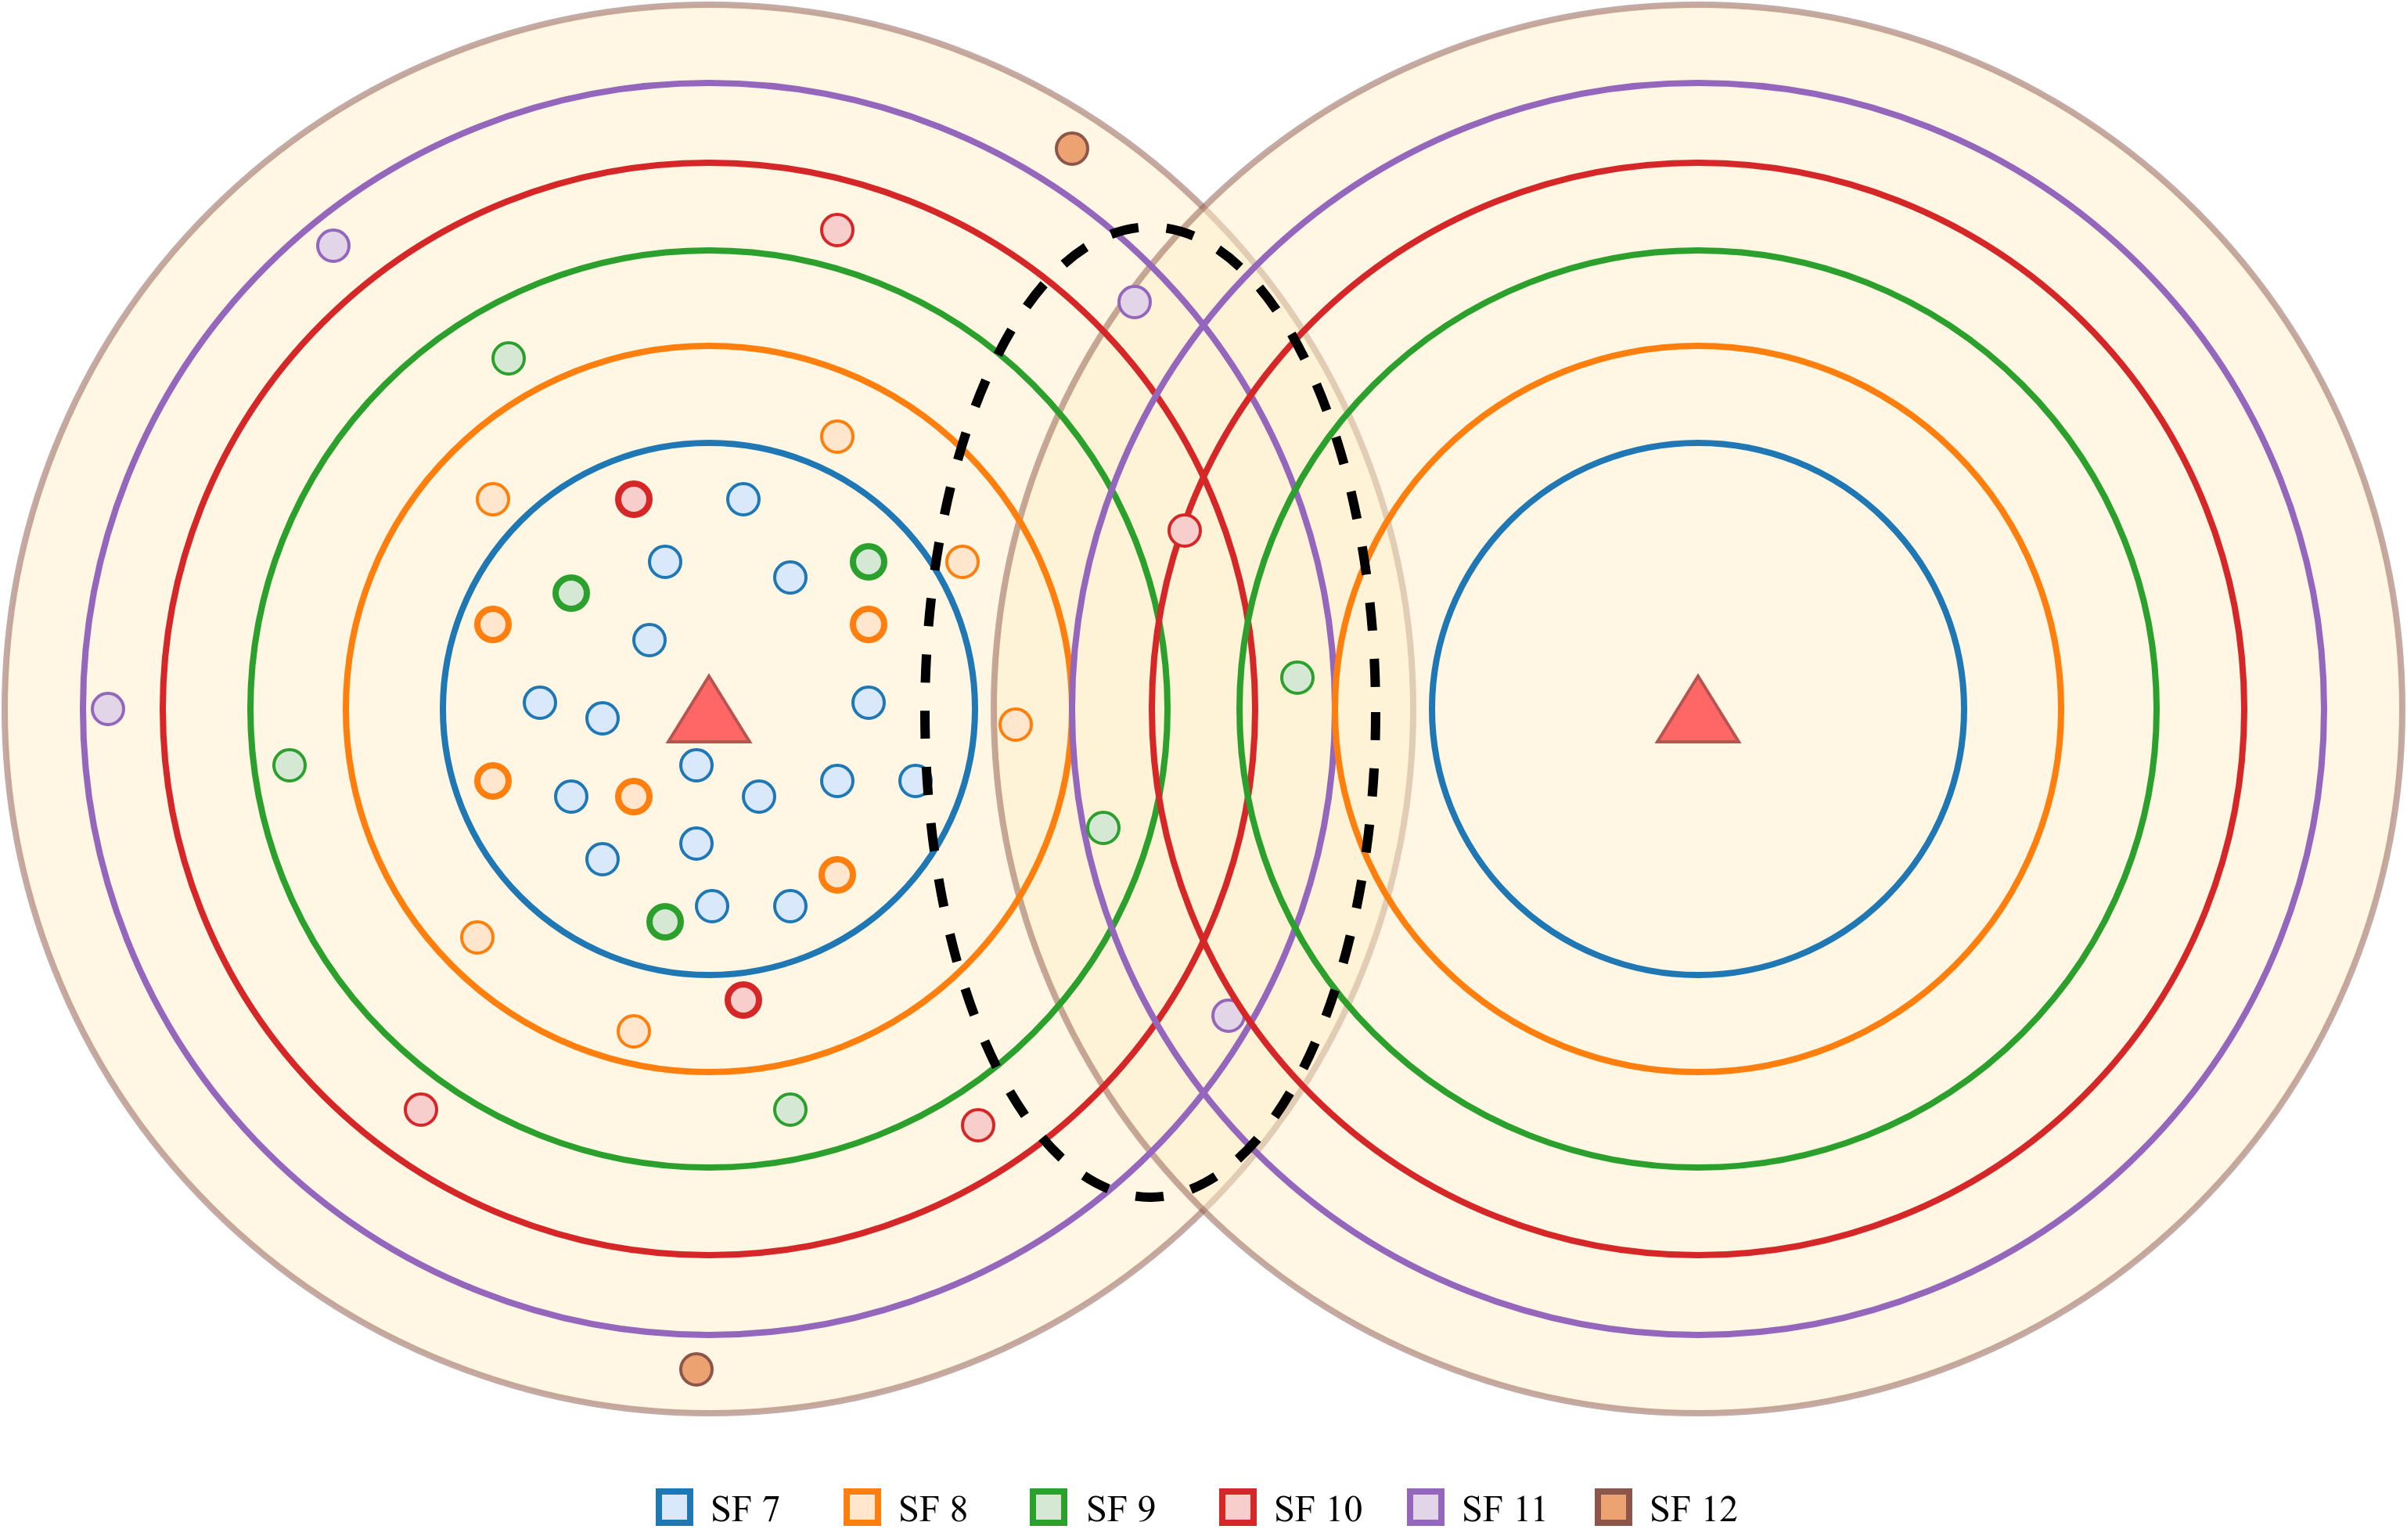
\includegraphics[width=0.5\textwidth]{collision_solution_multi_gw}
\caption{Collision prevention proposal for intersecting GWs.}
\label{fig:collision_solution_multi_gw}
\end{figure}


\section{Simulation Environment and Results} \label{Simulation Environment and Results}
\par A discrete event simulator is implemented in Python to study LoRa network performance. The LoRaWAN SF simulation tool is publicly available at https://github.com/tugrulyatagan/simlorafs.

Simulation Assumptions

\subsection{Link Model}
\par [TODO] 

The link budget of a wireless system or network is a measure of all the gains and losses from the transmitter, through the propagation channel, to the target receiver. Link budget of a wireless link can be calculated as:

\begin{equation} \label{eq:expected_rx_power}
P^{dBm}_{RX} = P^{dBm}_{TX} + G^{dB}_{SYS} - L^{dB}_{SYS} - L^{dB}_{PATH}
\end{equation}

\par Where, $P^{dBm}_{RX}$ is the expected receive power at the receiver. $P^{dBm}_{TX}$ is the transmit power. $G^{dB}_{SYS}$ is the system gains such as transmitter and receiver antenna gains. $L^{dB}_{SYS}$ is the system losses such as transmitter and receiver line, circuit, antenna losses. $L^{dB}_{PATH}$ is the propagation path loss between transmitter and receiver antennas.

\par Propagation loss can be calculated as:

\begin{equation} \label{eq:propagation_loss}
\begin{split}
P^{dB}_{PATH} = 40(1 - 4 \times 10^{-3} \times h){\log_{10} R|_{km}} \\
- 18 {\log_{10} h|_{m}} + 21 {\log_{10} f|_{MHz}} + 80
\end{split}
\end{equation}

\par Where $h$ is the gateway altitude and $f$ is the frequency of the signal. We assume that $h$ = 15 m and $f$ = 868 MHz, Propagation loss can be calculated as:

\begin{equation} \label{eq:propagation_loss_simplified}
P^{dB}_{PATH} = 120.5 + 37.6 {\log_{10} R|_{km}}
\end{equation}

\par Receive sensitivity of a LoRa gateway for different SFs and BWs can be found in Table \ref{table:gw_sf_sensitivity} \cite{SX1276}. Maximum TX power for European ISM band LoRa default channels can be found in Table \ref{table:max_tx_power}.

\begin{table}
\centering
\caption{Gateway Sensitivity for different SFs}
\label{table:gw_sf_sensitivity}
\begin{tabular}{|c|c|c|c|c|c|c|c|}
\hline
\multicolumn{2}{|c|}{\multirow{2}{*}{}} & \multicolumn{6}{c|}{\textbf{SF}} \\ \cline{3-8}
\multicolumn{2}{|c|}{}                  &    7 &    8 &    9 &   10 &   11 &   12 \\ \hline
\multirow{3}{*}{\textbf{BW}}  & 125 kHz & -123 & -126 & -129 & -132 & -133 & -136 \\ \cline{2-8}
                              & 250 kHz & -120 & -123 & -125 & -128 & -130 & -133 \\ \cline{2-8}
                              & 500 kHz & -116 & -119 & -122 & -125 & -128 & -130 \\ \hline
\end{tabular}
\end{table}

\begin{table}
\centering
\caption{EU863-870 ISM Band LoRa Default Channels}
\label{table:max_tx_power}
\begin{tabular}{|c|c|c|c|}
\hline
\textbf{Channel} & \textbf{Frequency} & \textbf{Bandwidth} & \textbf{Max EIRP} \\ \hline
      1 &     868.1 &   125 kHz &   14 dBm \\ \hline
      2 &     868.3 &   125 kHz &   14 dBm \\ \hline
      3 &     868.5 &   125 kHz &   14 dBm \\

\hline
\end{tabular}
\end{table}

\subsection{Interference Model}
\par [TODO]

\begin{equation} \label{eq:sinr}
T = \begin{bmatrix}
       6 & -16 & -18 & -19 & -19 & -20 \\
     -24 &   6 & -20 & -22 & -22 & -22 \\
     -27 & -27 &   6 & -23 & -25 & -25 \\
     -30 & -30 & -30 &   6 & -26 & -28 \\
     -33 & -33 & -33 & -33 &   6 & -29 \\
     -36 & -36 & -36 & -36 & -36 &   6
     \end{bmatrix}
\end{equation}

\begin{equation} \label{eq:sinr_db}
SINR_{i,j} = \dfrac{P_{rc,0}}{\sum_{l \in I_j} P_{rc,l}}
\end{equation}

\begin{equation} \label{eq:sinr_t}
SINR_{i,j}^{dB} > T_{i,j}
\end{equation}

\begin{equation} \label{eq:p_interference}
P_{rc,y}^{interf} = \dfrac{P_{rc,y}(T_{x}-t_{1})}{T_{x}}
\end{equation}

\begin{figure}
\centering
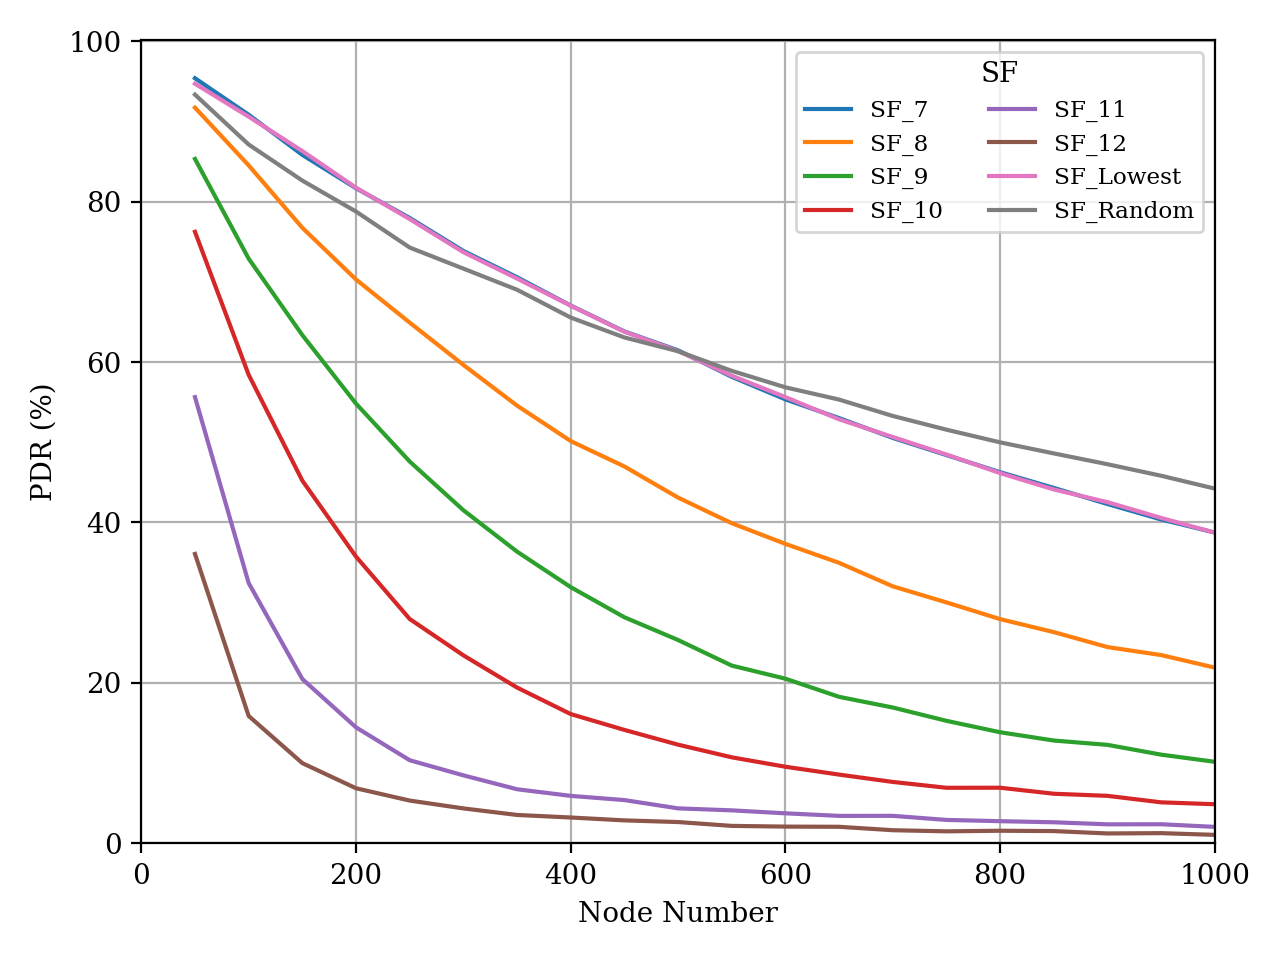
\includegraphics[width=0.5\textwidth]{sf_pdr}
\caption{PDR of different SFs.}
\label{fig:sf_pdr}
\end{figure}

\begin{figure}
\centering
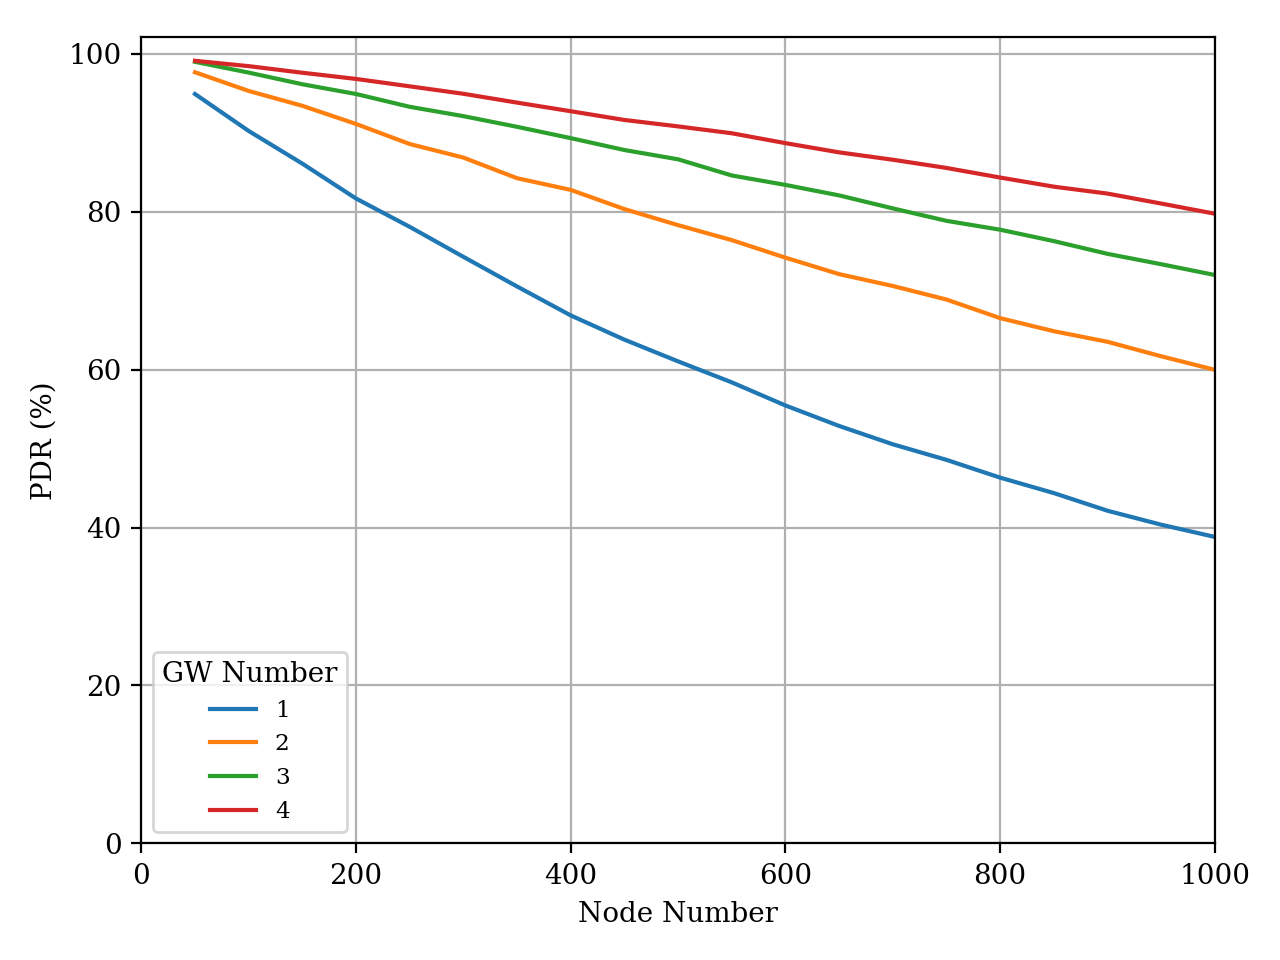
\includegraphics[width=0.5\textwidth]{gw_pdr}
\caption{PDR of different gateway numbers.}
\label{fig:gw_pdr}
\end{figure}

\begin{figure}
\centering
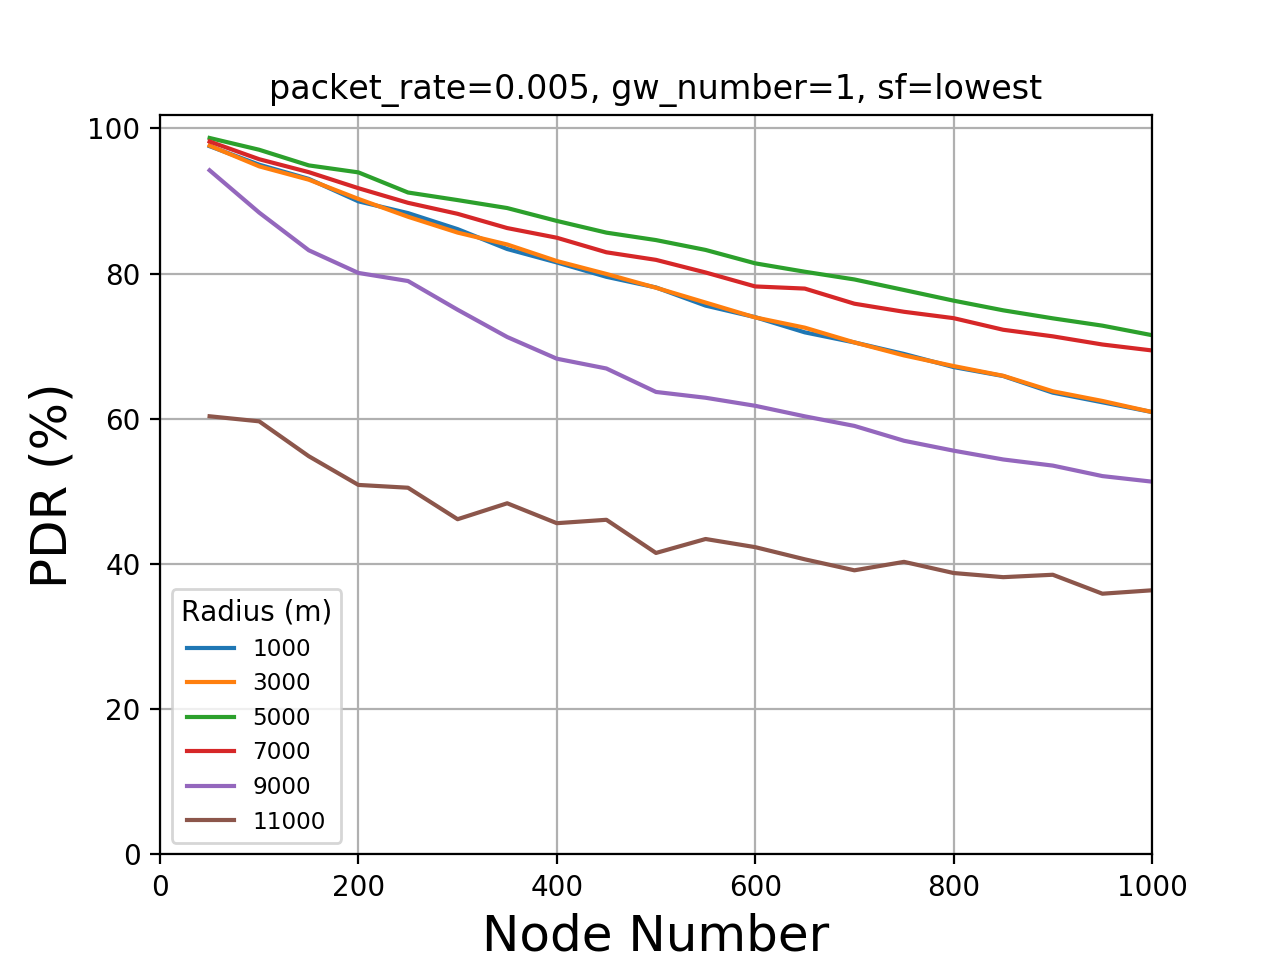
\includegraphics[width=0.5\textwidth]{r_pdr}
\caption{PDR of different topology radius.}
\label{fig:r_pdr}
\end{figure}

\begin{figure}
\centering
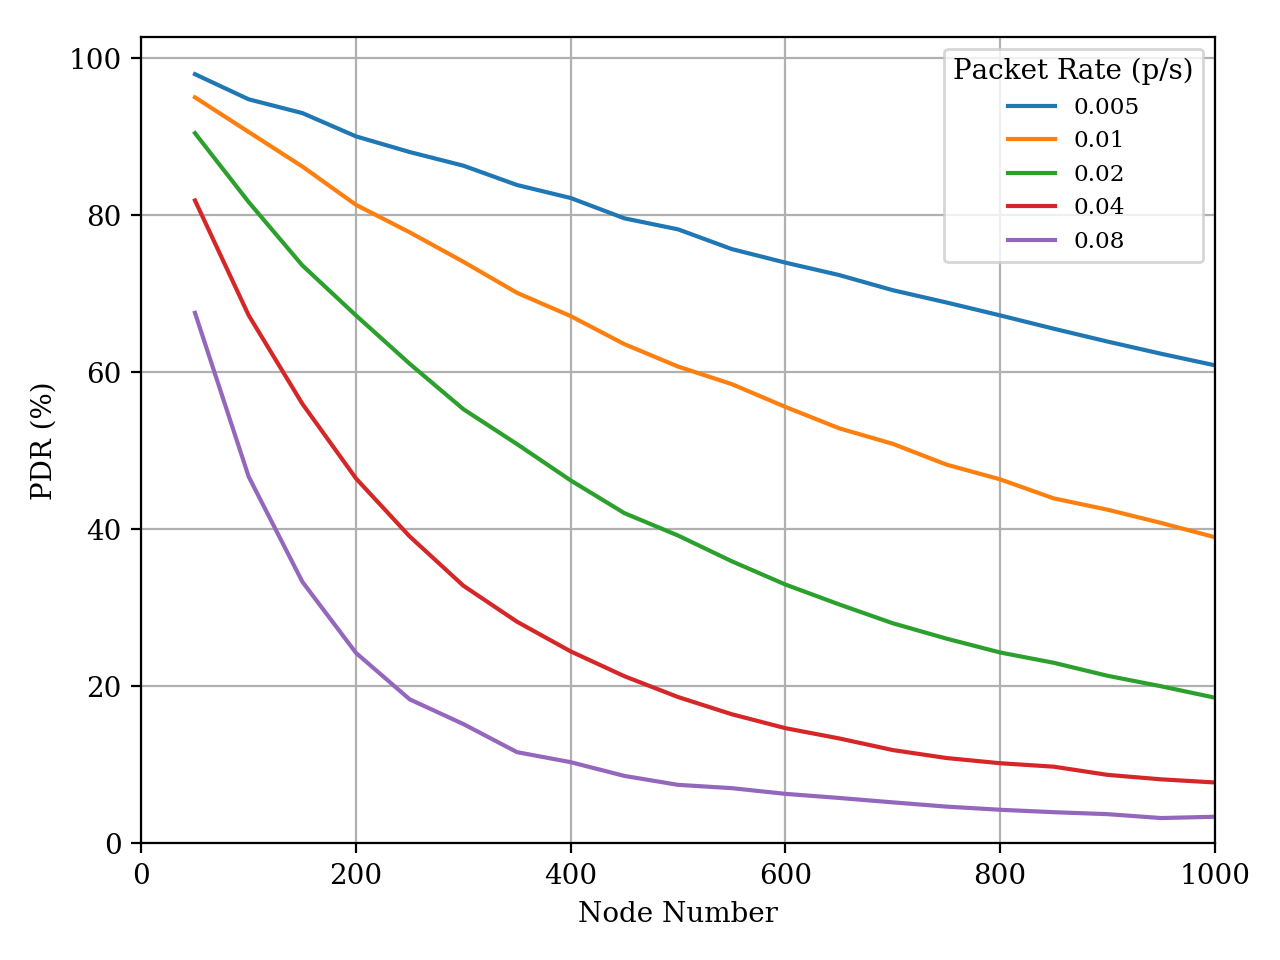
\includegraphics[width=0.5\textwidth]{pr_pdr}
\caption{PDR of different packet rates.}
\label{fig:pr_pdr}
\end{figure}

\begin{figure}
\centering
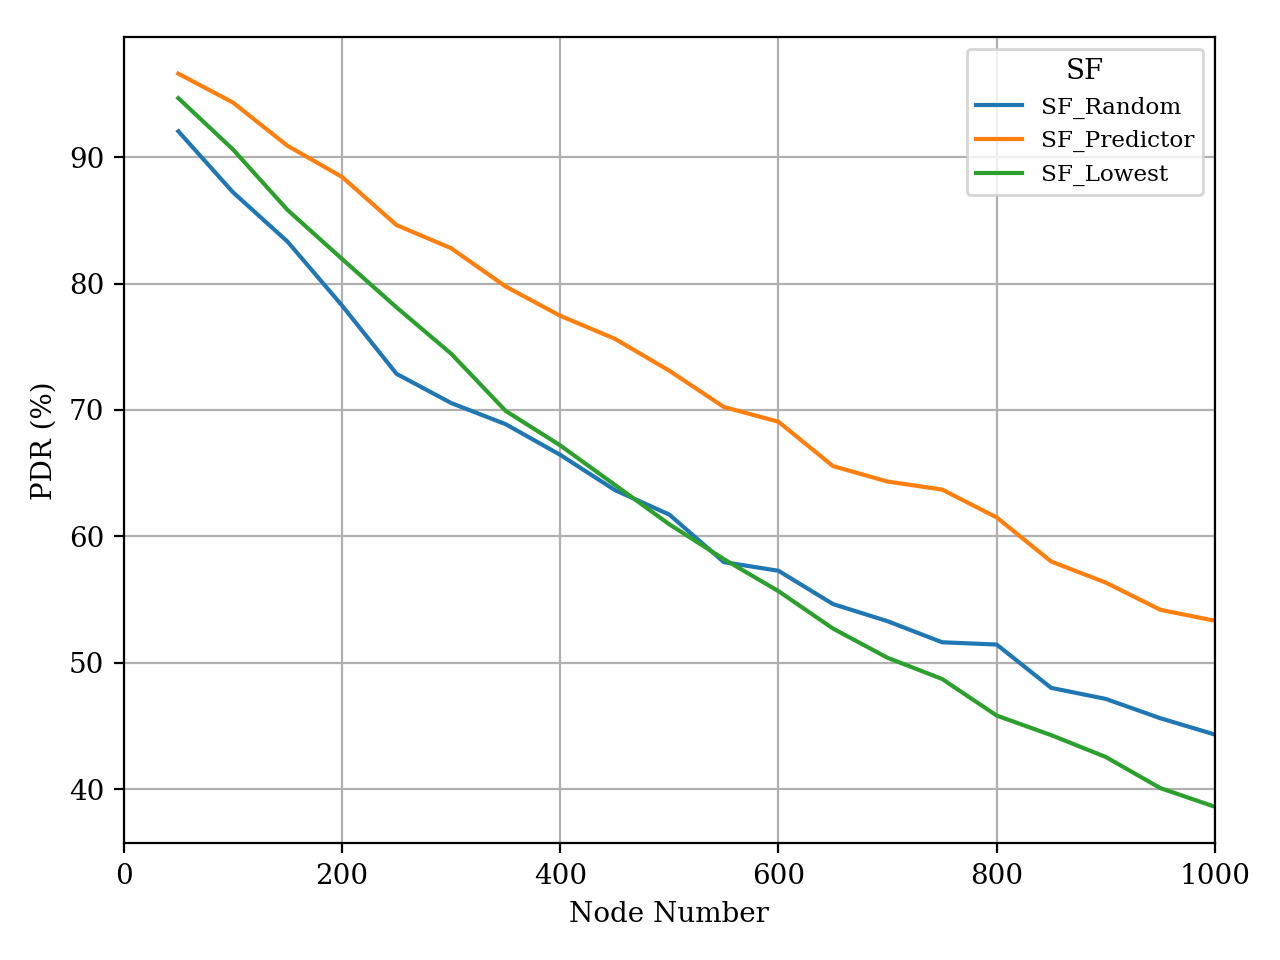
\includegraphics[width=0.5\textwidth]{predict_pdr}
\caption{PDR of different prediction SF assignment scheme.}
\label{fig:pr_pdr}
\end{figure}

\subsection{Simulation Results}
\par [TODO] Evaluation


\section{Conclusion} \label{Conclusion}
\par In this paper, after brief introduction about LPWAN technologies, we provide background information about one of the most promising LPWAN technology, LoRa. Then, we discuss about LoRa modulation basics and spreading factor assignment issue. We have implemented a discrete event simulator from scratch to study network performance of LoRaWAN and evaluate different SF assignment schemes. We have shown how same SF transmission collisions can be avoided and we proposed a machine learning based solution for collision with same SF transmissions. We illustrate simulation results for proposed machine learning SF assignment technique. Our simulation results show that, proposed technique can increase network performance up to [TBD] \%.

\par As for future works, transmit power optimization can be included to proposed machine learning scheme. In this paper, we assume nodes always uses maximum transmit power for uplink transmission, however nodes close to the GW can decrease transmit power to save energy. This will make transmission more vulnerable to interference thus requires extra care. Optimizing another node parameter alongside SF can be interesting research. Also other machine learning methods can be investigated for SF optimization. 
Reinforcement learning can be a good candidate for this network optimization issue.

\par \cite{7815384} \cite{7803607} \cite{7996384} \cite{8090518} \cite{s17061193} \cite{8267219} \cite{8430542} \cite{8319183} \cite{8480649} \cite{AN1200.22} \cite{Bor:2016:LLW:2988287.2989163} \cite{8406255} \cite{DBLP:journals/corr/abs-1802-10338} \cite{finnegan2018comparative}


\section*{Acknowledgment}
\par This work is supported by Turkish Ministry of Development and Istanbul Technical University researcher support program under the Grant No. ITU-AYP-2017-1.


\bibliographystyle{IEEEtran}
\bibliography{references}

\end{document}
